\documentclass[12pt]{article}

% essential packages
\usepackage[utf8]{inputenc}
\usepackage[french]{babel}
\usepackage[T1]{fontenc}

% other packages
\usepackage{packages}
\usepackage{multirow}

\usepackage{tikz}
\usetikzlibrary{shapes.geometric, arrows, positioning, arrows.meta, calc, external, automata}
\tikzexternalize
\tikzexternaldisable

\definecolor{forestgreen}{rgb}{0.0, 0.27, 0.13}

\title{Projet 4 -  RODD}
\date{\today}
\author{\textsc{BATY Léo}, \textsc{BRUNOD-INDRIGO Luca}}

\begin{document}

\maketitle

\section{Programme linéaire en variable mixtes}

\begin{maxie}|s|[2] % maxie = minimize 
    {x, d}  % optimization variables
    {w_1 \sum_{(i, j)\in M\times N} t_{ij}(1 - x_{ij}) + w_2 g l \sum_{(i, j)\in M\times N}4x_{ij} - d_{ij}} % objective function and label
    {\label{P1}} % label for optimization problem
    {} % optimization result
    \addConstraint{d_{ij}}{\geq \sum_{(k, l)\in A_{ij}}x_{kl} - |A_{ij}|(1 - x_{ij})\quad}{\forall (i, j)\in M\times N}
    \addConstraint{d_{ij}}{\in \bbR_+}{\forall (i, j)\in M\times N}
    \addConstraint{x_{ij}}{\in \{ 0, 1 \}}{\forall (i, j)\in M\times N}
\end{maxie}

\noindent Soit $(x, d)$ solution optimale de \ref{P1} :
\begin{bulletlist}
    \item $\sum\limits_{(i, j)\in M\times N} t_{ij}(1 - x_{ij})$ : population de l'espèce 1 (somme des $t_{ij}$ pour toutes les parcelles coupées)
    \item $g l \sum\limits_{(i, j)\in M\times N}4x_{ij} - d_{ij}$
    \begin{itemize}[label=$\bullet$]
        \item si $x_{ij} = 1$, $d_{ij} = \sum\limits_{(k, l)\in A_{ij}}x_{kl}$ nombre de voisins de $(i, j)$ non coupés
        Donc $4x_{ij} - d_{ij}$ est le nombre de lisières
        \item si $x_{ij} = 0$, $d_ij = 0$ et $4x_{ij} - d_{ij} = 0$
    \end{itemize}
\end{bulletlist}
Le modèle compte donc bien la somme pondérée de la population 1 et de la population 2.

\section{Programme linéaire quadratique en variables binaires}

\begin{maxie}|s|[2] % maxie = minimize 
    {x, d}  % optimization variables
    {w_1 \sum_{(i, j)\in M\times N} t_{ij}(1 - x_{ij}) + w_2 g l \sum_{(i, j)\in M\times N}\sum_{(k,l) \in A_{ij}}x_{ij}(1 - x_{kl})} % objective function and label
    {} % label for optimization problem
    {} % optimization result
    \addConstraint{x_{ij}}{\in \{ 0, 1 \}\quad}{\forall (i, j)\in M\times N}
\end{maxie}

\noindent On ajoute les contraintes de linéarisation (de type Fortet) suivantes : $y_{ijkl} = x_{ij}(1 - x_{kl})$
\begin{bulletlist}
    \item $y_{ijkl} \leq x_{ij}$
    \item $y_{ijkl} \leq 1 - x_{kl}$
    \item $y_{ijkl} \geq x_{ij} - x_{kl}$ (non nécessaire car on maximise avec des coefficients positifs)
    \item $y_{ijkl} \geq 0$ (non nécessaire car on maximise avec des coefficients positifs)
\end{bulletlist}

\noindent Ce qui donne :

\begin{maxie}|s|[2] % maxie = minimize 
    {x, d}  % optimization variables
    {w_1 \sum_{(i, j)\in M\times N} t_{ij}(1 - x_{ij}) + w_2 g l \sum_{(i, j)\in M\times N}\sum_{(k,l) \in A_{ij}}y_{ijkl}} % objective function and label
    {\label{P2}} % label for optimization problem
    {} % optimization result
    \addConstraint{y_{ijkl}}{\leq x_{ij}}{\forall (i, j)\in M\times N,\, \forall (k,l) \in A_{ij}}
    \addConstraint{y_{ijkl}}{\leq 1 - x_{kl}\quad}{\forall (i, j)\in M\times N,\, \forall (k,l) \in A_{ij}}
    \addConstraint{x_{ij}}{\in \{ 0, 1 \}\quad}{\forall (i, j)\in M\times N}
    \addConstraint{y_{ijkl}}{\in  \bbR}{\forall (i, j)\in M\times N,\, \forall (k,l) \in A_{ij}}
\end{maxie}

\noindent La matrice des contraintes de (\ref{P2}) est totalement unimodulaire (TU). En effet :
\begin{bulletlist}
    \item Elle est de la forme 
    $\begin{pmatrix}
        Id & M\\
    \end{pmatrix}$ avec $M$ de taille $M^2N^2\times MN$, et $$M_{ijkl, pq} = \1_{\{ pq = kl \}} - \1_{\{ pq = ij \}},\, \forall (i, j, k, l), (p, q)$$
    \item \textbf{Caractérisation de Ghouila-Houri} : soit $I$ un sous-ensemble de colonnes de $M$. On partitionne $I$ en $I_1 = I$ et $I_2 = \emptyset$. Pour chaque ligne, la somme des éléments de $I_1$ vaut $-1$, $0$, ou $1$ (par définition de $M$), et la somme des éléments de $I_2$ vaut $0$. La somme sur les lignes diffère d'au plus $1$, on conclut donc que $M$ est TU, donc que la matrice des contraintes est TU.
\end{bulletlist}

\noindent On peut donc enlever la contrainte d'intégrité des variables :

\begin{maxie}|s|[2] % maxie = minimize 
    {x, d}  % optimization variables
    {w_1 \sum_{(i, j)\in M\times N} t_{ij}(1 - x_{ij}) + w_2 g l \sum_{(i, j)\in M\times N}\sum_{(k,l) \in A_{ij}}y_{ijkl}} % objective function and label
    {} % label for optimization problem
    {} % optimization result
    \addConstraint{y_{ijkl}}{\leq x_{ij}}{\forall (i, j)\in M\times N,\, \forall (k,l) \in A_{ij}}
    \addConstraint{y_{ijkl}}{\leq 1 - x_{kl}\quad}{\forall (i, j)\in M\times N,\, \forall (k,l) \in A_{ij}}
    \addConstraint{x_{ij}}{\in [0, 1]\quad}{\forall (i, j)\in M\times N}
    \addConstraint{y_{ijkl}}{\in  \bbR}{\forall (i, j)\in M\times N,\, \forall (k,l) \in A_{ij}}
\end{maxie}

\section{Résultats}

\subsection{Instances de l'énoncé}

\noindent Voici les résultats obtenus pour les deux instances de l'énoncé :

\begin{table}[H]
    \centering
    \begin{tabular}{|c|c|c|c|c|c|}
    \hline
                        & \textbf{Objectif} & \textbf{Effectif e1} & \textbf{Effectif e2} & \textbf{Parcelles non coupeées} & \textbf{Lisières} \\ \hline
    \textbf{Instance 1} & 8219.5782         & 6630                 & 317.91564            & 21                              & 84                \\ \hline
    \textbf{Instance 2} & 442.55536         & 191                  & 60.55536             & 5                              & 16                \\ \hline
    \end{tabular}
    \caption{Solutions des deux instances}
    \label{tab:solutions}
\end{table}

\begin{center}
    \begin{tikzpicture}[scale=0.5, every node/.style={transform shape}]
        \tikzstyle{box} = [rectangle,draw=black,thick, minimum size=1cm]
    
        \foreach \x in {1,...,10}{
            \foreach \y in {1,...,10}
                \node[box] at (\x,\y){};
        }
        
        \node[box, fill=forestgreen!50] at (2,10){};
        \node[box, fill=forestgreen!50] at (9,10){};

        \node[box, fill=forestgreen!50] at (5,9){};
        \node[box, fill=forestgreen!50] at (8,9){};

        \node[box, fill=forestgreen!50] at (3,8){};
        \node[box, fill=forestgreen!50] at (6,8){};

        \node[box, fill=forestgreen!50] at (2,7){};
        \node[box, fill=forestgreen!50] at (5,7){};

        \node[box, fill=forestgreen!50] at (1,6){};
        \node[box, fill=forestgreen!50] at (3,6){};
        \node[box, fill=forestgreen!50] at (7,6){};
        \node[box, fill=forestgreen!50] at (10,6){};

        \node[box, fill=forestgreen!50] at (3,4){};
        \node[box, fill=forestgreen!50] at (7,4){};
        \node[box, fill=forestgreen!50] at (10,4){};

        \node[box, fill=forestgreen!50] at (2,3){};
        \node[box, fill=forestgreen!50] at (5,3){};
        \node[box, fill=forestgreen!50] at (9,3){};

        \node[box, fill=forestgreen!50] at (4,2){};

        \node[box, fill=forestgreen!50] at (5,1){};
        \node[box, fill=forestgreen!50] at (8,1){};
    
    \end{tikzpicture}
\end{center}

\begin{center}
    \begin{tikzpicture}[scale=0.5, every node/.style={transform shape}]
        \tikzstyle{box} = [rectangle,draw=black,thick, minimum size=1cm]
    
        \foreach \x in {1,...,5}{
            \foreach \y in {1,...,5}
                \node[box] at (\x,\y){};
        }

        \node[box, fill=forestgreen!50] at (4,5){};
        \node[box, fill=forestgreen!50] at (3,4){};
        \node[box, fill=forestgreen!50] at (3,3){};
        \node[box, fill=forestgreen!50] at (1,2){};
        \node[box, fill=forestgreen!50] at (1,1){};
    \end{tikzpicture}
\end{center}

\noindent Voici un tableau comparatif des deux modèles :

\begin{table}[H]
    \centering
    \begin{tabular}{|c|c|c|c|c|}
    \hline
    \multirow{2}{*}{\textbf{Modèle}} & \multicolumn{2}{c|}{\textbf{Instance 1}}         & \multicolumn{2}{c|}{\textbf{Instance 2}}         \\ \cline{2-5} 
                                     & \textbf{Temps de calcul} & \textbf{Nb de noeuds} & \textbf{Temps de calcul} & \textbf{Nb de noeuds} \\ \hline
    \textbf{Modèle 1}             & 0.01 s                   & 0                     & 0.013 s                  & 0                     \\ \hline
    \textbf{Modèle 2}               & 0.004 s                  & n.a.                  & 0.0014 s                 & n.a.                  \\ \hline
    \end{tabular}
    \caption{Résultats pour les deux instances de l'énoncé}
    \label{tab:results}
\end{table}

\subsection{Ajout d'une contrainte sur le nombre de parcelles non coupées}


\noindent On ajoute la contrainte suivante $\sum\limits_{(i, j)\in M\times N} x_{ij} \geq 60$ (au moins $60$ parcelles non coupées). On obtient les résultats suivants pour les deux méthodes
\begin{table}[H]
    \centering
    \begin{tabular}{|c|c|c|c|c|}
    \hline
                        \textbf{Objectif} & \textbf{Effectif e1} & \textbf{Effectif e2} & \textbf{Parcelles non coupeées} & \textbf{Lisières} \\ \hline
                        6753.933200000012         & 3272                 & 696.38664           & 60                              & 184                \\ \hline
    \end{tabular}
    \caption{Solutions des deux instances}
\end{table}


\begin{center}
    \begin{tikzpicture}[scale=0.5, every node/.style={transform shape}]
        \tikzstyle{box} = [rectangle,draw=black,thick, minimum size=1cm]
    
        \foreach \x in {1,...,10}{
            \foreach \y in {1,...,10}
                \node[box] at (\x,\y){};
        }
        
        \node[box, fill=forestgreen!50] at (1,10){};
        \node[box, fill=forestgreen!50] at (2,10){};
        \node[box, fill=forestgreen!50] at (5,10){};
        \node[box, fill=forestgreen!50] at (6,10){};
        \node[box, fill=forestgreen!50] at (7,10){};
        \node[box, fill=forestgreen!50] at (8,10){};
        \node[box, fill=forestgreen!50] at (9,10){};
        \node[box, fill=forestgreen!50] at (10,10){};

        \node[box, fill=forestgreen!50] at (1,9){};
        \node[box, fill=forestgreen!50] at (3,9){};
        \node[box, fill=forestgreen!50] at (5,9){};
        \node[box, fill=forestgreen!50] at (7,9){};
        \node[box, fill=forestgreen!50] at (9,9){};

        \node[box, fill=forestgreen!50] at (2,8){};
        \node[box, fill=forestgreen!50] at (4,8){};
        \node[box, fill=forestgreen!50] at (6,8){};
        \node[box, fill=forestgreen!50] at (8,8){};
        \node[box, fill=forestgreen!50] at (10,8){};

        \node[box, fill=forestgreen!50] at (1,7){};
        \node[box, fill=forestgreen!50] at (3,7){};
        \node[box, fill=forestgreen!50] at (5,7){};
        \node[box, fill=forestgreen!50] at (7,7){};
        \node[box, fill=forestgreen!50] at (9,7){};

        \node[box, fill=forestgreen!50] at (1,6){};
        \node[box, fill=forestgreen!50] at (2,6){};
        \node[box, fill=forestgreen!50] at (4,6){};
        \node[box, fill=forestgreen!50] at (6,6){};
        \node[box, fill=forestgreen!50] at (8,6){};
        \node[box, fill=forestgreen!50] at (10,6){};

        \node[box, fill=forestgreen!50] at (1,5){};
        \node[box, fill=forestgreen!50] at (3,5){};
        \node[box, fill=forestgreen!50] at (5,5){};
        \node[box, fill=forestgreen!50] at (7,5){};
        \node[box, fill=forestgreen!50] at (9,5){};

        \node[box, fill=forestgreen!50] at (1,4){};
        \node[box, fill=forestgreen!50] at (2,4){};
        \node[box, fill=forestgreen!50] at (4,4){};
        \node[box, fill=forestgreen!50] at (6,4){};
        \node[box, fill=forestgreen!50] at (8,4){};
        \node[box, fill=forestgreen!50] at (10,4){};

        \node[box, fill=forestgreen!50] at (1,3){};
        \node[box, fill=forestgreen!50] at (3,3){};
        \node[box, fill=forestgreen!50] at (5,3){};
        \node[box, fill=forestgreen!50] at (7,3){};
        \node[box, fill=forestgreen!50] at (9,3){};
        \node[box, fill=forestgreen!50] at (10,3){};
        
        \node[box, fill=forestgreen!50] at (2,2){};
        \node[box, fill=forestgreen!50] at (4,2){};
        \node[box, fill=forestgreen!50] at (6,2){};
        \node[box, fill=forestgreen!50] at (8,2){};
        \node[box, fill=forestgreen!50] at (10,2){};

        \node[box, fill=forestgreen!50] at (1,1){};
        \node[box, fill=forestgreen!50] at (3,1){};
        \node[box, fill=forestgreen!50] at (5,1){};
        \node[box, fill=forestgreen!50] at (6,1){};
        \node[box, fill=forestgreen!50] at (7,1){};
        \node[box, fill=forestgreen!50] at (8,1){};
        \node[box, fill=forestgreen!50] at (9,1){};
        \node[box, fill=forestgreen!50] at (10,1){};
    
    \end{tikzpicture}
\end{center}


\noindent \textbf{Remarque} : on obtient les mêmes solutions pour les deux méthodes, cependant l'ajout de la nouvelle contrainte fait perdre la caractère TU de la matrice des contraintes du second modèle. En effet, on ajoute une ligne composée de $-1$ à $M$, ce qui permet d'identifier un sous-déterminant $\begin{vmatrix}
    -1 & 1\\
    -1 & -1
    \end{vmatrix} = 2\notin \{ 0, 1, -1\}$. En général, on est donc pas sûr que le PL du second modèle renvoie une solution entière.

\subsection{Instances aléatoires}

\noindent Voici un plot du temps de calcul en fonction de la taille de l'instance pour les deux méthodes :

\begin{figure}[H]
    \centering
    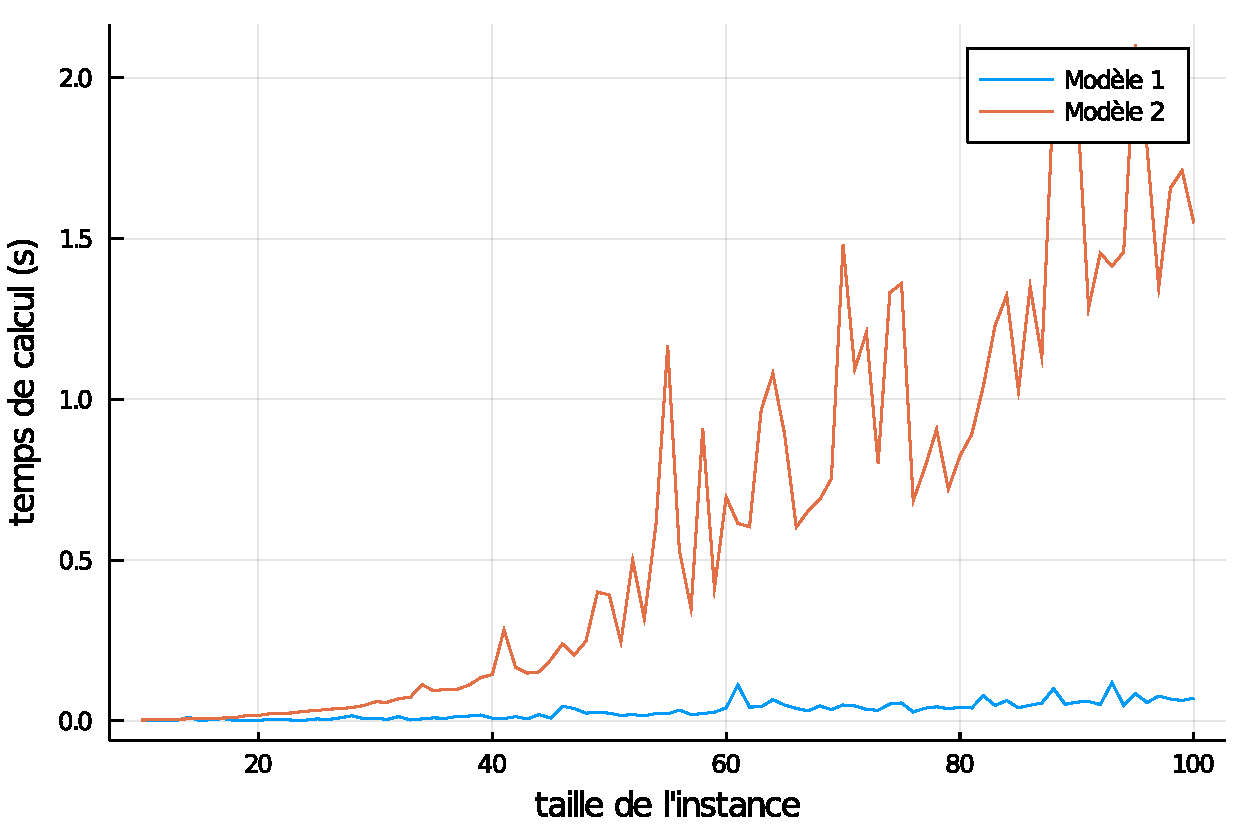
\includegraphics[width=10cm]{fig1.pdf}
\end{figure}

\noindent Le modèle 1 semble beaucoup plus efficace que le modèle 2.

\end{document}